\documentclass[a4paper, 14pt]{extarticle}
\usepackage{enumitem}
\usepackage{fefutitle}
\usepackage{listings}
\usepackage{xcolor}
\usepackage{amsmath}
\usepackage{graphicx}
\usepackage[justification=centering]{caption}
\usepackage{float}

\lstdefinestyle{mystyle}{
	basicstyle={\small\ttfamily},
	keywordstyle=\color{orange},
	stringstyle=\color{green},
	basicstyle=\ttfamily\footnotesize,
	breakatwhitespace=false,         
	breaklines=true,                 
	captionpos=b,                    
	keepspaces=true,                 
	numbers=none,                    
	numbersep=5pt,                  
	showspaces=false,                
	showstringspaces=false,
	showtabs=false,                  
	tabsize=2,
	aboveskip=3mm,
	belowskip=3mm,
}
\lstset{style=mystyle}

\begin{document}
	\fefutitle{2}{Модель нагревательного прибора}
	\pagebreak	

	\section{Введение}
		В данной лабораторной необходимо создать модель нагревательного прибора. В качестве прибора возьмём электрический утюг, так как это элемент бытовой техники, который есть практически у всех. Утюг был изобретен давно. Например, до появления электричества существовали угольные утюги.	
		
 		Но с появлением электричества и развития техники, появились электрические утюги. Работа электрического утюга с электрическим нагревом основана на выделении тепловой энергии при прохождении электрического тока через нагревательный элемент. Температура нагревательного элемента сообщается подошве утюга, которая также нагревается. Ранние электрические утюги не имели регулировки температуры и их было необходимо отключать от сети при достижении небходимой температуры. Температура современных электрических утюгов задается отдельным терморегулятором, главная функция которого заключается в своевременном отключении подачи электроэнергии в соответствии с заданным режимом.
		
		\begin{figure}[H]
			\centering
			\includegraphics[width = .5\linewidth]{utug.jpg}
			\caption[.] {Современный электрический утюг}
		\end{figure}
	
		Основной характеристикой является мощность.

	\section{Создание математической модели}
		Количество теплоты(\(\Delta Q\)), которое получает утюг при увеличении его температуры на величину 
		\( \Delta T = T_2 - T_1 \) вычисляется так:
		\[ \Delta Q = cm \Delta T \], где \( T_1, T_2\) - температуры утюга до нагрева и после.
		
		Количество теплоты, отдаваемое утюгом в окружающую среду вычисляется по закону Ньютона-Рихмана:
		\[ Q = kS(T-T_a) \Delta t \]
		, где \(k\) - коэффициент теплообмена, $T_a = 293K = 20^{\circ}C$ - температура окружающей среды,
		$c$ - удельная темплоёмкость подошвы утюга, $S$ - площадь поверхности подошвы, $T$ - температура утюга
			
		Нагретый утюг излучают энергию в виде электромагнитных волн различной длины. Тепловое излучение:
		\[ E = \sigma T^4 \]
		, где \( \sigma = 5.67 \cdot 10^{-8} \) - постоянная Стефана-Больцмана
		
		Составим уравнение теплового баланса:
		\[ \Delta Q = P\Delta t - kS(T-T_a) \Delta t - S \sigma T^4 \Delta t +  S \sigma T_a^4 \Delta t\],
		$P$ - мощность утюга, $\Delta t$ - время работы утюга
		
		\[ cm \Delta T = P\Delta t - kS(T-T_a) \Delta t - S \sigma (T^4 - T_a) \Delta t \]
		
		Поделим на \( \Delta t\) и умножим на \(cm\)
		\[ \dfrac{\Delta T}{\Delta t} 
		= \dfrac{P - kS(T-T_a) - S \sigma T^4 +  S \sigma T_a^4}{cm}\]
		
		Перейдём к дифференциальному уравнению и добавим начальное условие(в начальный момент времени
		температура подошвы утюга равна температуре окружающей среды):
		\[
			\begin{cases}
				\dfrac{dT}{dt} = \dfrac{P - kS(T-T_a) - S \sigma (T^4 - T_a)}{cm},\\
				T(0) = T_a.
			\end{cases} \tag{1} \label{eq:1}
		\]
		
		Для утюга с терморегулятором добавим функцию, которая будет отвечать за включение и отключение утюга
		после достижения заданной максимальной температуры $T_{max}$
		\[ H(T) = 
			\begin{cases}
				0, \text{если} T \geq T_{max}\\
				1, \text{если} T \leq T_{min}
			\end{cases} 
		\]
		
		Тогда дифференциальное уравнение примет следующий вид:
		\[
		\begin{cases}
			\dfrac{dT}{dt} = \dfrac{ P\cdot H(T) - kS(T-T_a) - S \sigma (T^4 - T_a)}{cm},\\
			T(0) = T_a.
		\end{cases} \tag{2} \label{eq:2}
		\]
	
	\section{Реализация модели}
		\setlength\parindent{0pt}
		Программы были написаны на языке Java. Для решение дифференциального уравнения
		использовался метод Эйлера, который имеет первый порядок точности.
		\subsection{Утюг без терморегулятора}
			Код программы:
			\begin{lstlisting}[language=Java]
public class Main {
	private static final Integer T0 = 291;
	private static Integer state = HEATING;
	
	private static class Func implements Function<Double, Double> {
		@Override
		public Double apply(Double T) {
			double sigma = 5.67E-8;
			int P = 1600;
			int c = 900;
			double m = 0.8;
			double s = 0.02;
			int k = 25;
			return (P - k * s *(T - T0) - s * sigma *(Math.pow(T, 4) - Math.pow(T0, 4))) / c * m;
		}
	}
	
	private static ArrayList<Double> euler(Function<Double, Double> func, ArrayList<Integer> t) {
		ArrayList<Double> res = new ArrayList<>();
		
		double T = T0.doubleValue();
		for (int tValue: t) {
			T += func.apply(T);
			res.add(T);
		}
		return res;
	}
	
	public static void main(String[] args) throws PythonExecutionException, IOException {
		ArrayList<Integer> t = new ArrayList<>();
		for(int i = 0; i <= 1000; ++i) {
			t.add(i);
		}
		
		ArrayList<Double> T = euler(new Func(), t);
	}
}
			\end{lstlisting}
			\begin{figure}[H]
				\centering
				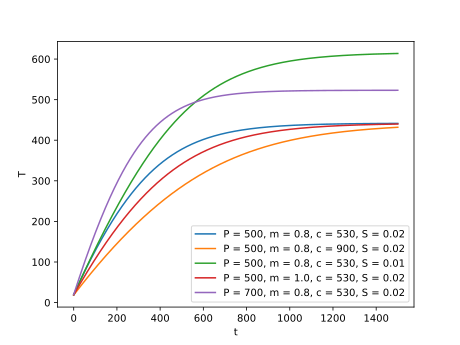
\includegraphics[width = .75\linewidth]{fig1.pdf}
				\caption[.] {График решения дифференциального уравнения \eqref{eq:1} при разных данных}
			\end{figure}
		\pagebreak
		\subsection{Утюг с терморегулятором}
			Код программы:
			\begin{lstlisting}[language=Java]
public class Main {
	private static final Integer COOLING = 0;
	private static final Integer HEATING = 1;
	private static final Integer T0 = 291;
	private static final Integer T_max = 483;
	private static final Integer T_min = 453;
	private static Integer state = HEATING;
	private static Integer thermostat(double T) {
		if (T >= T_max) {
			state = COOLING;
		} else if (T <= T_min) {
			state = HEATING;
		}
		return state.equals(COOLING) ? 0 : 1;
	}
	private static class Func implements Function<Double, Double> {
		@Override
		public Double apply(Double T) {
			double sigma = 5.67E-8;
			int P = 2000;
			int c = 900;
			double m = 0.8;
			double s = 0.02;
			int k = 25;
			return (P * thermostat(T)- k * s *(T - T0) - s * sigma *(Math.pow(T, 4) - Math.pow(T0, 4))) / (c * m);
		}
	}
	
	private static ArrayList<Double> euler(Function<Double, Double> func, ArrayList<Integer> t) {
		ArrayList<Double> res = new ArrayList<>();
		
		double T = T0.doubleValue();
		for (int tValue: t) {
			T += func.apply(T);
			res.add(T);
		}
		return res;
	}
	
	public static void main(String[] args) throws PythonExecutionException, IOException {
		ArrayList<Integer> t = new ArrayList<>();
		for(int i = 0; i <= 1500; ++i) {
			t.add(i);
		}
		
		ArrayList<Double> T = euler(new Func(), t);
	}
}
			\end{lstlisting}
			\begin{figure}[H]
				\centering
				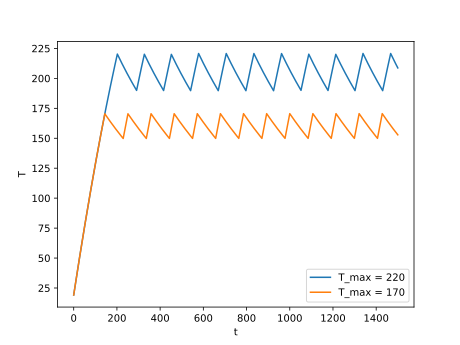
\includegraphics[width = .65\linewidth]{fig2.pdf}
				\caption[.] {График решения дифференциального уравнения \eqref{eq:2} 
				при $P = 500$ Вт, $m = 0.8$ кг, $c = 530$ Дж/К, $S = 0.02 \text{м}^2$}
			\end{figure}
			
			\begin{figure}[H]
				\centering
				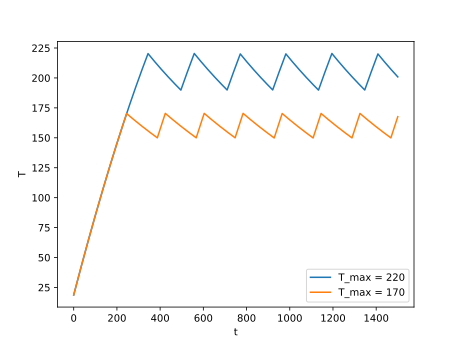
\includegraphics[width = .65\linewidth]{fig3.pdf}
				\caption[.] {График решения дифференциального уравнения \eqref{eq:2} 
					при $P = 500$ Вт, $m = 0.8$ кг, $c = 900$ Дж/К, $S = 0.02 \text{м}^2$ }
			\end{figure}
			
			\begin{figure}[H]
				\centering
				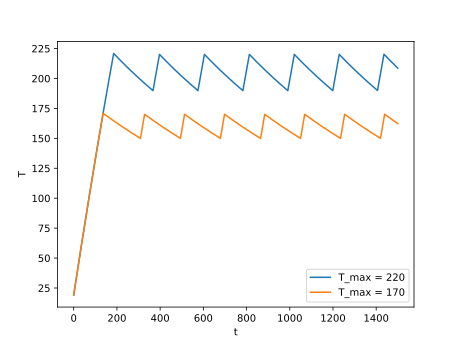
\includegraphics[width = .65\linewidth]{fig4.pdf}
				\caption[.] {График решения дифференциального уравнения \eqref{eq:2} 
					при $P = 500$ Вт, $m = 0.8$ кг, $c = 530$ Дж/К, $S = 0.01 \text{м}^2$}
			\end{figure}
			
			\begin{figure}[H]
				\centering
				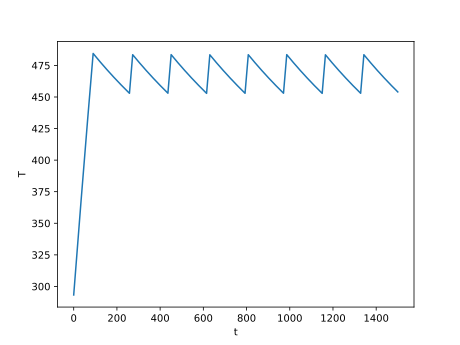
\includegraphics[width = .65\linewidth]{fig5.pdf}
				\caption[.] {График решения дифференциального уравнения \eqref{eq:2} 
					при $P = 500$ Вт, $m = 1$ кг, $c = 530$ Дж/К, $S = 0.02 \text{м}^2$}
			\end{figure}
			
			\begin{figure}[H]
				\centering
				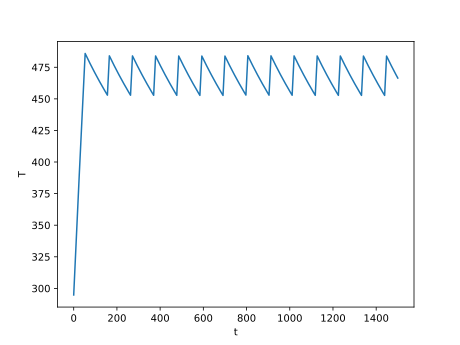
\includegraphics[width = .65\linewidth]{fig6.pdf}
				\caption[.] {График решения дифференциального уравнения \eqref{eq:2} 
					при $P = 700$ Вт, $m = 0.8$ кг, $c = 530$ Дж/К, $S = 0.02 \text{м}^2$}
			\end{figure}
			
	\section{Вывод}
		Таким образом, построена математическая модель утюга с терморегулятором и без него. Она позволяет получить график температур от времени для утюгов с различными площадями подошвы, теплопроводностями и мощностями. 
		
\end{document}	